\NeedsTeXFormat{LaTeX2e}

\documentclass[12pt]{article}
\usepackage[letterpaper,portrait, margin=1in]{geometry}
\usepackage{booktabs, pgfplots, bm, multirow, amsmath, wrapfig, gensymb, graphicx}
\pgfplotsset{width=11cm,compat=1.9}
\renewcommand{\arraystretch}{1.5}
\usepackage[colorlinks=true, allcolors=blue]{hyperref}
\usepackage{indentfirst}



\begin{document}

%%%%%%%%%%%%%%%%%%%%%%%%%%%%%%%%%%%%%%%%%%%%%%%%%%%%%%%%%%%%
%%% COVER PAGE - TO BE COPIED AT BEGINNING OF LAB REPORT %%%
%%%      PLEASE ALSO FILL OUT WITH YOUR INFORMATION      %%%
%%%%%%%%%%%%%%%%%%%%%%%%%%%%%%%%%%%%%%%%%%%%%%%%%%%%%%%%%%%%

\begin{titlepage}

       %\vspace*{.5cm}
        \begin{center}
        \textbf{\huge PH-291 Physics Lab} \\ 
        \textbf{\Large Professor Corn-Agostini} \\ 
        \textbf{\Large Fall 2022} \\ 
        \vspace*{.5cm}  
        \textbf{\large Lab \# 4: Optical Instruments}
        \vspace{0.5cm}
        \end{center}
       
\noindent Your Name:\\ \\
\noindent Your Lab Section:\\ \\
\noindent Your Lab Instructor:\\ \\
\noindent Your Lab Partner's Name:\\ \\
\noindent Read and sign Academic Integrity Statement:\\

\noindent {\em I hereby attest that I have not given or received any unauthorized assistance on this assignment.}

    \begin{center}
    \line(1,0){300} \\
    Sign here
    \end{center}

\noindent\textbf{\large Grading Rubric} \\ \\
\renewcommand{\arraystretch}{1.5}
%\large
\begin{tabular}{|l|c|r|l|} \hline
 {\bf CATEGORY} & {\bf POINTS} & {\bf GRADE}\\\hline 
Purpose & 2 & \\\hline
Data & 6 & \\\hline
Theory \& Calculations (includes Q1 and Q2) & 6 & \\\hline 
Results \& Analysis & 4 & \\\hline 
Conclusion  & 2 & \\\hline \hline 
{\em Total} & 20 & \\ \hline
\end{tabular}

\end{titlepage} 

\end{document}


\newpage
\tableofcontents
\newpage
\section{Purpose}
In this lab, Bessel's Method will be used to determine the focal lengths of two converging lenses. 
The focal length of each length is approximated using the thin lens equation (Eq. 1). 
Here, the lenses are convex, meaning that $f$ is positive.
This approximate focal length is used to determine the distance between the source and the screen $(D)$. 
$D$ must be sufficiently large so that the light rays will converge and form a real image. 
If $D$ is too small, a virtual image will be formed, which only exists within the brain.
A clear image is formed by each lens in two positions, the difference of which $(d)$ is used in Bessel's Method to calculate the focal lengths.
The angular magnification of the two lenses will then be calculated and used to construct a simple telescope, which is used to test the expected magnification value.  
\newpage
\section{Data}
\begin{center}
    \begin{minipage}{.5\linewidth}
        \centering
        \begin{tabular}{|c | c|}
            \hline
            \textbf{Measurement} & \textbf{Thickness (mm)}  \\ \hline
            1 & 1.695 \\ 
            2 & 1.995 \\ 
            3 & 1.990  \\ 
            4 & 2.095 \\ 
            5 & 1.930 \\ 
            6 & 1.995 \\ \hline
            \multicolumn{2}{|c|}{\textbf{Instrumental Error:} 0.005 mm} \\
            \multicolumn{2}{|c|}{\textbf{Random Error:} 0.055 mm} \\
            \multicolumn{2}{|c|}{\textbf{Thickness:} $1.950\pm0.055$ mm} \\ \hline
        \end{tabular}
        \vspace{3mm}
        \\Table 1: Petri Dish Thickness
        \vspace{10mm}
    \end{minipage}%
    \begin{minipage}{.5\linewidth}
        \centering
        \begin{tabular}{|c | c|}
            \hline
            \textbf{Measurement} & \textbf{Thickness (mm)}  \\ \hline
            1 & 7.98 \\ 
            2 & 8.86 \\ 
            3 & 8.24  \\ 
            4 & 7.60 \\ 
            5 & 8.16 \\ 
            6 & 7.66 \\ \hline
            \multicolumn{2}{|c|}{\textbf{Instrumental Error:} 0.02 mm} \\
            \multicolumn{2}{|c|}{\textbf{Random Error:} 0.19 mm} \\
            \multicolumn{2}{|c|}{\textbf{Thickness:} $8.08\pm0.19$ mm} \\ \hline
        \end{tabular}
        \vspace{3mm}
        \\Table 2: Ring Diameter Without Liquid
        \vspace{10mm}
    \end{minipage} 
    \begin{tabular}{|c|c|}
        \hline
        \textbf{Measurement} & \textbf{Diameter (mm)} \\ \hline
        1 & 19.68 \\ 
        2 & 19.60 \\ 
        3 & 19.58 \\ 
        4 & 19.58 \\ 
        5 & 19.56 \\ 
        6 & 19.62 \\ \hline
        \multicolumn{2}{|c|}{\textbf{Instrumental Error:} 0.02 mm} \\
        \multicolumn{2}{|c|}{\textbf{Random Error:} 0.017 mm} \\
        \multicolumn{2}{|c|}{\textbf{Thickness:} $19.60\pm0.02$ mm} \\ 
        \hline
    \end{tabular}
    \vspace{3mm}
    \\Table 3: Ring Diameter With Liquid
    \begin{tabular}{|c|c c|}
    \hline
        \textbf{Measurement} & \textbf{Incident Angle} & \textbf{Refracted Angle} \\ \hline
        1 & $50.0\degree$ & $28.0\degree$ \\ 
        2 & $28.0\degree$ & $38.0\degree$ \\ 
        3 & $36.0\degree$ & $20.0\degree$ \\ 
        4 & $17.0\degree$ & $40.0\degree$ \\ 
        5 & $43.0\degree$ & $27.0\degree$ \\ 
        6 & $28.0\degree$ & $39.0\degree$ \\ \hline
        \multicolumn{3}{|c|}{\textbf{Instrumental Error:} $0.5\degree$} \\ \hline
    \end{tabular}
    \vspace{3mm}
    \\Table 4: Snell's Law
\end{center}
\newpage
\section{Calculations}
\subsection*{Part A: Bessel's Method for Determining Focal Length}
\noindent \textbf{1. Thin Lens Equation}\[\frac{1}{p}+\frac{1}{i}=\frac{1}{f}\]
    Where $p$ is the distance between the source and the lens, $i$ is the distance between the image and the lens, and $f$ is the focal length of the lens. \\
\textbf{2. Focal Length of Lens $\bm{({f})}$}\[f=\frac{D^2-d^2}{4D}\]
    Initially, the focal length of each lens is approximated, which allows us to find our value for $D$, the distance between the source and screen. $D$ must be greater than $4f$, where $f$ is our approximate focal length. Each lens has two positions where a sharp image is displayed, and the difference between these two positions provides our $d$ value. From there, an accurate focal length can be determined for each lens using this equation.
    The error of the mean values were propagated through this calculation using the following equations.
\subsubsection*{Error Propagation:}
    \noindent\textbf{2.1 Partial Derivative of Eq. 2 w.r.t $\bm d$}\[\frac{\partial f}{\partial d}=\dfrac{-d}{2D}\]
    \textbf{2.2 Partial Derivative of Eq. 2 w.r.t $\bm D$} \[\frac{\partial f}{\partial D}=\dfrac{D^2+d^2}{4D^2}\]
    Each of these partial derivatives are used in the final calculation of the total error associated with $f.$ Because $d$ and $D$ are dependent variables we use the following equation to find the total error.\\
    \textbf{2.3 Total Error Associated with the Focal Length $\bm{(f)}$}\[\delta f =\left|\frac{\partial f}{\partial d}\delta d\right|+\left|\frac{\partial f}{\partial D}\delta D\right|\]
    The error associated with the mean values were calculated (shown in Tables 6 and 7). This provides our final error associated with $f$.\\
\\\textbf{3. Angular Magnification $\bm{(m_\theta)}$}\[m_\theta=-\frac{f_{obj}}{f_{eye}}\]
    We proceed to calculate the angular magnification $(m_\theta)$, which relies on the focal lengths of both lenses. $f_{obj}$ is the focal length of the objective lens, which is the lens with a longer focal length. The lens with the short focal length acts as the eyepiece, $f_{eye}.$ The total error of $m_\theta$ is found using the following equations.
\subsubsection*{Error Propagation:}
    \noindent\textbf{3.1 Partial Derivative of Eq. 3 w.r.t $\bm f_{obj}$}\[\frac{\partial m_\theta}{\partial f_{obj}}=\dfrac{-1}{f_{eye}}\]
    \textbf{3.2 Partial Derivative of Eq. 3 w.r.t $\bm f_{eye}$} \[\frac{\partial m_\theta}{\partial f_{eye}}=\dfrac{f_{obj}}{f_{eye}^2}\]
    Each of these partial derivatives are used in calculating the total error in the following equation. Both $f_{eye}$ and $f_{obj}$ are independent, which allows us to use the following equation.\\
    \textbf{3.3 Total Error Associated with the Angular Magnification $\bm{({m_\theta})}$}\[\delta m_\theta =\sqrt{\left(\frac{\partial m_\theta}{\partial f_{obj}}\delta f_{obj}\right)^2+\left(\frac{\partial m_\theta}{\partial f_{eye}}\delta f_{eye}\right)^2}\]
    As in Equation 1.3, this equation gives us the total error associated with $(m_\theta)$, shown in the results section (Table 8).
\newpage
\section{Results}
\begin{center}
    \centering
    \begin{tabular}{|c|c|c|c|}
    \hline
        $n_\text{glass}$ & $\frac{\partial n_\text{glass}}{\partial t}$ & $\frac{\partial n_\text{glass}}{\partial d}$ & Error of $n_\text{glass}$ \\ \hline
        1.39 & 0.34 & -0.08 & 0.08 \\ \hline
        \multicolumn{4}{|c|}{$\bm{n_\textbf{glass}: 1.39\pm0.08}$}\\\hline
    \end{tabular}
    \vspace{3mm}
    \\ Table 5: $n_\text{glass}$ Final Value by Pfund's Method\\
    \vspace{5mm}
    \centering
    \begin{tabular}{|c|c|c|c|c|c|}
    \hline
        $n_\text{liquid}$ & $\frac{\partial n_\text{liquid}}{\partial t}$ & $\frac{\partial n_\text{liquid}}{\partial d}$ & $\frac{\partial n_\text{liquid}}{\partial n_{\text{glass}}}$ & Error of $n_\text{glass}$ & Error of $n_\text{liquid}$ \\ \hline
        1.29 & -0.09 & 0.009 & 0.93 & 0.08 & 0.26 \\ \hline
        \multicolumn{6}{|c|}{$\bm{n_\textbf{liquid}: 1.29\pm0.26}$}\\\hline
    \end{tabular} 
    \vspace{3mm}
    \\ Table 6: $n_\text{liquid}$ Final Value by Pfund's Method\\
    \vspace{5mm} 
    \centering
    \begin{tabular}{|c|c|c|c|}
    \hline
        $n_\text{liquid}$ & $\frac{\partial n_\text{liquid}}{\partial \theta_1}$ & $\frac{\partial n_\text{liquid}}{\partial \theta_2}$  & Error of $n_\text{liquid}$ \\ \hline
        1.62 & 1.88 & -3.82 & 0.04  \\ \hline
        \multicolumn{4}{|c|}{$\bm{n_\textbf{liquid}: 1.62\pm0.04}$}\\\hline
    \end{tabular} 
    \vspace{3mm}
    \\ Table 7: $n_\text{liquid}$ Final Value by Snell's Law\\
    \vspace{5mm}
    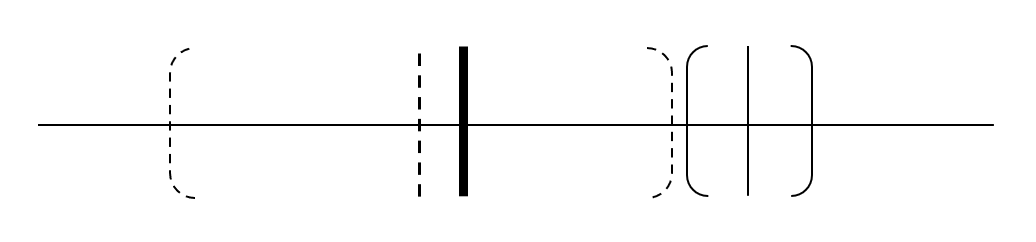
\includegraphics[scale=0.5]{number line.png}\\
    Dashed = Method 1 (Pfund's Method)\\
    Solid = Method 2 (Snell's Law)\\
    Bold = Accepted Value \\
    Figure 1: Number Line Indicating Error Bounds and Accepted Values   
\end{center}
Using Figure 1, we can see that while the index of refraction calculated via Pfund's Method had a greater error, it was closer to the accepted value of the index of refraction of water, which is 1.33. The accepted index of refraction lies within the error bounds of the Pfund's Method calculation. Snell's method provided an index of refraction of $1.62\pm0.04$ which does not agree with the accepted value. This can mainly be attributed to human error in measuring the incident and refracted angles. When measuring our angles, we misread our protractor as having increments at every $1\degree$, as opposed to every $0.5\degree$. This provided us with an instrumental error of $0.5\degree$, as opposed to $0.25\degree$.
\\\indent The error introduced in Pfund's Method stems from multiple areas. Firstly, the petri dish may not have had a uniform thickness, providing different thickness readings on the micrometer. Then, the laser may not have been pointed perfectly vertically. Pfund's method relies on the laser making an angle of $\frac{\pi}{2}$ with the horizontal. Lastly, error is introduced in measuring each of the rings. The method of measuring required eyeballing where the ring lined up on the polar grid and then measuring the polar grid on a separate piece of paper. Measurements were taken using a pair of vernier calipers, which have pointed ends where the measurements are taken. These tended to make indentations in the polar grid paper which the calipers would slide into when taking other measurements.\\
\indent The second method using Snell's Law had less error associated with the final index of refraction relative to the value found by Pfund's Method. The calculated index of refraction is $1.62\pm0.04$. While tracing the petri dish onto our surface, the polar grid on the bottom of the dish caused us to trace a larger circle than the diameter of the petri dish. Then, when placing the pins along the path of the laser, the laser may have been nudged out of position. This would affect the accuracy of our measured angles. The center of the circle may also have been misplaced, as it is found using the perpendicular bisectors of two cords. These perpendicular bisectors may not have been exactly perpendicular. This would affect the measurements taken for our angles, and in turn affect our index of refraction.
\newpage
\section{Conclusion}
Using Bessel's method, a focal length for Lens F1 was calculated to be $5.00\pm0.03$ cm, and $9.83\pm0.03$ cm for Lens C. 
These calculated focal lengths provided a magnification factor of $1.965\pm0.014$. 
Based on the calculated magnification factor and focal lengths, a simple telescope was constructed, which provided an experimental magnification factor of $2.11\pm0.05$. 
Although these magnification factors do not lie in the same error range, further experimental measurements could provide more similar experimental and theoretical magnification factors.
The difference between the experimental and theoretical values can b attributed to human error, as described above. 
If error could be reduced, Bessel's Method will provide for more accurate focal length and magnification factor values.
\newpage
\section{Questions}
\subsection*{1. Derive the equation $\bm{f=\frac{D^2-d^2}{4D}}$ and explain why we need the subsidiary condition $\bm{D>4f}$.}
\noindent Starting with the thin lens equation (Eq. 1), \[\frac{1}{p}+\frac{1}{i}=\frac{1}{f}\] Since $i$ is the distance between the image and the lens, we can rewrite the equation, \[i=D-p\]\[\frac{1}{p}+\frac{1}{D-p}=\frac{1}{f}\] 
We then rewrite as the following equation \[Df=pD-p^2\] which can be solved via the quadratic equation \[p=\frac{D\pm\sqrt{D^2-4Df}}{2}\]
Note here that if $D>4f$ the discriminant is positive, meaning that for all other cases an imaginary answer will be given for $p$. We can denote the two positions of $p$ by $d$, which is the difference between the two positions
\[d=\frac{D+\sqrt{D^2-4Df}}{2}-\frac{D-\sqrt{D^2-4Df}}{2}=\sqrt{D^2-4fD}\]
Using this value of $d$, we can solve for $f$ \[d^2=D^2-4fD\]\[D^2-d^2=4fD\]
\[\boxed{f=\frac{D^2-d^2}{4D}}\]
\newpage
\subsection*{2. To get the approximate focal length of the lens we approximated the distance from the lens to the source to be infinite when it was actually finite (but large). Use the thin lens equation to show that this will slightly overestimate the focal length of the lens.}
\noindent Starting with the thin lens equation (Eq. 1), \[\frac{1}{p}+\frac{1}{i}=\frac{1}{f}\]
Since we take $p\rightarrow\infty$, $\frac{1}{p}\rightarrow0$, which provides us with the following relationship\[0+\frac{1}{i}=\frac{1}{f}\Rightarrow f=i\]
Substituting back into the thin lens equation gives \[\frac{1}{p}+\frac{1}{f}=\frac{1}{f}\] which implies that a finite $p$ value will make for a slight overestimation of the focal length.
\end{document}